%%%%%%%%%%%%%%%%%%%%%%%%%%%%%%%%%%%%%%%%%%%%%%%%%%%%%%%%%%%%%%%%%%%%%%%%%%%%%%
% Report
% LaTeX Template
% Version 1.0 (December 8 2014)
%
% This template has been downloaded from:
% http://www.LaTeXTemplates.com
%
% Original author:
% Brandon Fryslie
% With extensive modifications by:
% Vel (vel@latextemplates.com)
%
% License:
% CC BY-NC-SA 3.0 (http://creativecommons.org/licenses/by-nc-sa/3.0/)
%
%%%%%%%%%%%%%%%%%%%%%%%%%%%%%%%%%%%%%%%%%%%%%%%%%%%%%%%%%%%%%%%%%%%%%%%%%%%%%%

\documentclass[usletter, 11pt]{extarticle}
%%%%%%%%%%%%%%%%%%%%%%%%%%%%%%%%%%%%%%%%%
% Contract Structural Definitions File Version 1.0 (December 8 2014)
%
% Created by: Vel (vel@latextemplates.com)
% 
% This file has been downloaded from: http://www.LaTeXTemplates.com
%
% License: CC BY-NC-SA 3.0 (http://creativecommons.org/licenses/by-nc-sa/3.0/)
%
%%%%%%%%%%%%%%%%%%%%%%%%%%%%%%%%%%%%%%%%%

\usepackage{geometry} % Required to modify the page layout
\usepackage{multicol}
\usepackage{amsmath}
\usepackage{amssymb}

\usepackage[pdftex]{graphicx}
\usepackage{wrapfig}
\usepackage[font=scriptsize, labelfont=bf]{caption}
\usepackage[utf8]{inputenc} % Required for including letters with accents
\usepackage[T1]{fontenc} % Use 8-bit encoding that has 256 glyphs

\usepackage{avant} % Use the Avantgarde font for headings
\usepackage{courier}
\usepackage{xparse}
\usepackage{xcolor}
\usepackage{listings}  % for code verbatim and console outputs

\setlength{\textwidth}{16cm} % Width of the text on the page
\setlength{\textheight}{23cm} % Height of the text on the page
\setlength{\oddsidemargin}{0cm} % Width of the margin - negative to move text left, positive to move it right
\setlength{\topmargin}{-1.25cm} % Reduce the top margin

\setlength{\parindent}{0mm} % Don't indent paragraphs
\setlength{\parskip}{2.5mm} % Whitespace between paragraphs
\renewcommand{\baselinestretch}{1.5}

\definecolor{green}{rgb}{0.18, 0.55, 0.34}

\graphicspath{ {figures/} }
\captionsetup[table]{skip=10pt}

\lstset{language=C, keywordstyle={\bfseries \color{black}}}

% defines algorithm counter for chapter-level
\newcounter{nalg}[section]

%defines appearance of the algorithm counter
\renewcommand{\thenalg}{\thesection .\arabic{nalg}}

% defines a new caption label as Algorithm x.y
\DeclareCaptionLabelFormat{algocaption}{Algorithm \thenalg}

% defines the algorithm listing environment
\lstnewenvironment{pseudocode}[1][] {
    \refstepcounter{nalg}  % increments algorithm number
    \captionsetup{font=normalsize, labelformat=algocaption, labelsep=colon}
    \lstset{
        breaklines=true,
        mathescape=true,
        numbers=left,
        numberstyle=\scriptsize,
        basicstyle=\footnotesize\ttfamily,
        keywordstyle=\color{black}\bfseries,
        keywords={input, output, return, parallel, function, for, to, in, if,
        else, foreach, while, and, or, new, print},
        xleftmargin=.04\textwidth,
        #1
    }
}{}

\renewcommand{\familydefault}{\sfdefault}  % default font for entire document
  % document layout and style

\newcommand{\project}{Project 2: Multithread LCS}
\newcommand{\members}{Sabbir Ahmed}
\newcommand{\V}[1]{\textup{#1}}
\newcommand{\lcs}{\V{lcs}}
\newcommand{\seqone}{\V{X}}
\newcommand{\seqtwo}{\V{Y}}
\newcommand{\lcsstr}{\V{lcsstr}}

\begin{document}

    \begin{titlepage}

        \vspace*{\fill} % Add whitespace above to center the title page content
        \begin{center}

            {\LARGE \project~Final Report}\\ [1.5cm]

            \today

            \vspace*{\fill}

            \members

        \end{center}
        \vspace*{\fill} % Add whitespace below to center the title page content

    \end{titlepage}

    \section{Description} The longest common subsequence (LCS) problem is to be
    implemented for the assignment. The objective of this project is to design,
    analyze, and implement a multithreaded version of the LCS length algorithm.
    A memoized or bottom-up approach. In either case, the goal is to design an
    algorithm that makes efficient use of multiple processors.

    Analysis is required once the LCS length algorithm is designed. The work
    $T_{1}(m, n)$ and the span $T_{\infty}(m, n)$ are to be computed, where $m$
    and $n$ are the lengths of the input sequences $X$ and $Y$, respectively.
    Finally, the parallelism is to be computed along with an estimate of a
    range of parameters ($m$, $n$, and $P$) for which linear or near-linear
    speed-up may be expected.

    The last part of the project is to implement the LCS length algorithm in C
    or C++ using OpenMP on UMBC's maya cluster and measure its performance
    empirically using 1, 2, 4, and 8 processors (optionally, it may be tested
    on 16 processors; most maya nodes have eight cores, but some have 16). Test
    data and LCS lengths of various sizes are to be generated to demonstrate
    the performance characteristics of the algorithm. The algorithm to recover
    the LCS must also be implemented, but this need not be multithreaded.

    \section{Initialization} The matrix is initialized to store the LCS before
    computation. Since the implementation utilizes a two-dimensional array
    allocated on the heap to represent the matrix, initialization was possible
    in $\Theta(m)$ time. Since Milestone 2, the initialization loop was
    parallelized to bring the runtime down to $\Theta(\text{lg}(m))$. This
    method is faster than iterating through all the cells of the matrix to
    assign each to a placeholder. Algorithm \thesection .\ref{alg1} provides
    the implementation used to initialize the matrix.

    Reading the sequences from the one-line input files, truncating them if
    necessary and storing them into buffers all take constant time operations.
    \newpage

\begin{pseudocode}[caption={Initialization of the Longest Common Subsequence
Matrix}, label={alg1}]
lcs_matrix = pointer array(m + 1);
parallel for i = 0 to m + 1
    $\lcs_{i}$ = pointer array(n + 1);

\end{pseudocode}

    \section{Serial Algorithm} Milestone 1 required implementation of the
    serial LCS length algorithm and its analysis. Table \ref{table:serialmat}
    visualizes the serial implementation of computing the LCS length of sample
    strings using the algorithm described in equation (15.9) of
    \textit{Introduction to Algorithms} \cite{Cormen:2009:IAT:1614191}.

\begin{table}[h]
    \caption{LCS matrix constructed when comparing \texttt{GCGTCA} and
    \texttt{ACGAA}} \label{table:serialmat}
    \centering
    \setlength\tabcolsep{0pt}
    \begin{tabular}{|@{\rule[-0.5cm]{0pt}{1cm}}*{8}{M{1cm} |}}
    \hline
    & \tikzmark{0}{$\bm{\varnothing}$} & \tikzmark{0}{\textbf{G}} &
    \tikzmark{0}{\textbf{C}} & \tikzmark{0}{\textbf{G}} &
    \tikzmark{0}{\textbf{T}} & \tikzmark{0}{\textbf{C}} &
    \tikzmark{0}{\textbf{A}} \\
    \hline
    \tikzmark{0}{$\bm{\varnothing}$} & \tikzmark{a0}{0} & \tikzmark{a1}{0} &
    \tikzmark{a2}{0} & \tikzmark{a3}{0} & \tikzmark{a4}{0} & \tikzmark{a5}{0} &
    \tikzmark{a6}{0} \\
    \hline
    \tikzmark{0}{\textbf{A}} & \tikzmark{b0}{0} & \tikzmark{b1}{0} &
    \tikzmark{b2}{0} & \tikzmark{b3}{0} & \tikzmark{b4}{0} & \tikzmark{b5}{0} &
    \tikzmark{b6}{1} \\
    \hline
    \tikzmark{0}{\textbf{C}} & \tikzmark{c0}{0} & \tikzmark{c1}{0} &
    \tikzmark{c2}{1} & \tikzmark{c3}{1} & \tikzmark{c4}{1} & \tikzmark{c5}{1} &
    \tikzmark{c6}{1} \\
    \hline
    \tikzmark{0}{\textbf{G}} & \tikzmark{d0}{0} & \tikzmark{d1}{1} &
    \tikzmark{d2}{1} & \tikzmark{d3}{2} & \tikzmark{d4}{2} & \tikzmark{d5}{2} &
    \tikzmark{d6}{2} \\
    \hline
    \tikzmark{0}{\textbf{A}} & \tikzmark{e0}{0} & \tikzmark{e1}{1} &
    \tikzmark{e2}{1} & \tikzmark{e3}{2} & \tikzmark{e4}{2} & \tikzmark{e5}{2} &
    \tikzmark{e6}{3} \\
    \hline
    \tikzmark{0}{\textbf{A}} & \tikzmark{f0}{0} & \tikzmark{f1}{1} &
    \tikzmark{f2}{1} & \tikzmark{f3}{2} & \tikzmark{f4}{2} & \tikzmark{f5}{2} &
    \tikzmark{f6}{3} \\
    \hline
    \end{tabular}

    \link{b1}{b0}
    \link{b2}{b1}
    \link{b3}{b2}
    \link{b4}{b3}
    \link{b5}{b4}
    \link{b6}{a5}

    \link{c1}{c0}
    \link{c2}{b1}
    \link{c3}{c2}
    \link{c4}{c3}
    \link{c5}{b4}
    \link{c6}{c5}

    \link{d1}{c0}
    \link{d2}{d1}
    \link{d3}{c2}
    \link{d4}{d3}
    \link{d5}{d4}
    \link{d6}{d5}

    \link{e1}{d1}
    \link{e2}{e1}
    \link{e3}{d3}
    \link{e4}{e3}
    \link{e5}{e4}
    \link{e6}{d5}

    \link{f1}{e1}
    \link{f2}{f1}
    \link{f3}{e3}
    \link{f4}{f3}
    \link{f5}{f4}
    \link{f6}{e5}

\end{table}

    \vspace{-0.5in}
    In Milestone 2, it was observed that the value of the cells depended on the
    cells above, left or top-left of itself. The cells in the other directions
    have no effect. This property allowing for subproblems to be independently
    solvable builds the foundation for the algorithm for the parallel
    implementation to find the LCS length.

    Algorithm \thesection .\ref{alg2} provides the pseudocode for
    computing the length of the LCS. The serial algorithm utilizes the bottom-up approach to compute the LCS.

\newpage
\begin{pseudocode}[caption={Serial Longest Common Subsequence Length},
label={alg2}]
function LCS-LENGTH(X, Y, m, n)
    // allocate (m + 1) $\times$ (n + 1) LCS matrix
    lcs = new matrix[1, 2, .., m + 1][1, 2, .., n + 1]
    for i = 0 to m
        for j = 0 to n
            // if upper-leftmost cell, content is 0
            if (i == 0 or j == 0)
                $\lcs_{i, j}$ = 0
            // if equal, content is the left anti-diagonal value incremented by 1
            else if ($\seqone_{i - 1}$ == $\seqtwo_{j - 1}$)
                $\lcs_{i, j}$ = $\lcs_{i-1, j-1}$ + 1  
            // maximum between previous row and previous column values
            else
                $\lcs_{i, j}$ = max($\lcs_{i-1, j}$, $\lcs_{i, j-1}$)
    return $\lcs_{m,n}$  // the last value of the matrix is the length

\end{pseudocode}

        % \vspace{-1in}
        \subsection{Time Complexity - Work} The running time of the serial
        implementation provides the work, $T_{1}$, of the algorithm. Simple
        analysis of the algorithm provided in the snippet Algorithm \thesection
        .\ref{alg2} suggests a non-linear running time from the nested loop.
        The inner loop (line 5) iterates $n$ times with several constant
        conditional checks, while the outer loop (line 4) iterates $m$ times.
        The runtime is therefore:
        \begin{equation*}
            \begin{split}
                T_1(m, n) & = \Theta(mn) \\
            \end{split}
        \end{equation*}

        The work for the algorithm, $\Theta(mn)$, is quadratic if $m = n$.

        \subsection{Printing the Longest Common Subsequence} After computing
        the length, the matrix may be used to print the LCS itself. Printing
        the subsequence is done in a serial implementation since the project
        does not emphasize its analysis. Since its implementation is not
        necessary for the scope of the project, the LCS printing functionality
        will be used for debugging purposes only. Algorithm \thesection
        .\ref{alg3} provides the pseudocode used to print the LCS.

\begin{pseudocode}[caption={Serial Longest Common Subsequence Printing},
label={alg3}]
function SERIAL-LCS-PRINT(X, Y, m, n, lcs)
    lcsstr = new string
    cursor = $\lcs_{m,n}$ // cursor of the matrix
    i = m, j = n // init from the bottom-rightmost cell
    while (i > 0 and j > 0)
        // if current character in X[] and Y[] are same
        if ($\seqone_{i - 1}$ == $\seqtwo_{j - 1}$)
            $\lcsstr_{cursor - 1}$ = $\seqone_{i - 1}$  // result gets current character
            i--, j--, cursor-- // decrement i, j and cursor
        // find the larger of two and go to that direction
        else if ($\lcs_{i - 1, j}$ > $\lcs_{i,j - 1}$)
            i--
        else
            j--
    print lcsstr

\end{pseudocode}

    \section{Parallel Algorithm} Milestone 2 required implementation of the
    parallel LCS length algorithm. This version of the implementation uses the
    same LCS matrix to generate the same cell values. Table
    \ref{table:serialmatsubprob} revisits the matrix generated by the serial
    implementation and highlights the independent subproblems.
    \newpage

\begin{table}[h]
    \caption{LCS matrix constructed when comparing \texttt{GCGTCA} and
    \texttt{ACGAA} with the anti-diagonal subproblems highlighted}
    \label{table:serialmatsubprob}
    \centering
    \setlength\tabcolsep{0pt}

    \begin{tabular}{|@{\rule[-0.5cm]{0pt}{1cm}}*{8}{M{1cm} |}}
        \hline
        & \tikzmark{0}{$\bm{\varnothing}$} & \tikzmark{0}{\textbf{G}} &
        \tikzmark{0}{\textbf{C}} & \tikzmark{0}{\textbf{G}} &
        \tikzmark{0}{\textbf{T}} & \tikzmark{0}{\textbf{C}} &
        \tikzmark{0}{\textbf{A}} \\

        \hline

        \tikzmark{0}{$\bm{\varnothing}$} &
        \cellcolor{Apricot!25}\tikzmark{a0}{0} &
        \cellcolor{Aquamarine!25}\tikzmark{a1}{0} &
        \cellcolor{BlueViolet!25}\tikzmark{a2}{0} &
        \cellcolor{BrickRed!25}\tikzmark{a3}{0} &
        \cellcolor{Goldenrod!25}\tikzmark{a4}{0} &
        \cellcolor{Fuchsia!25}\tikzmark{a5}{0} &
        \cellcolor{MidnightBlue!25}\tikzmark{a6}{0} \\

        \hline

        \tikzmark{0}{\textbf{A}} & \cellcolor{Aquamarine!25}\tikzmark{b0}{0} &
        \cellcolor{BlueViolet!25}\tikzmark{b1}{0} &
        \cellcolor{BrickRed!25}\tikzmark{b2}{0} &
        \cellcolor{Goldenrod!25}\tikzmark{b3}{0} &
        \cellcolor{Fuchsia!25}\tikzmark{b4}{0} &
        \cellcolor{MidnightBlue!25}\tikzmark{b5}{0} &
        \cellcolor{YellowOrange!25}\tikzmark{b6}{1} \\

        \hline

        \tikzmark{0}{\textbf{C}} & \cellcolor{BlueViolet!25}\tikzmark{c0}{0} &
        \cellcolor{BrickRed!25}\tikzmark{c1}{0} &
        \cellcolor{Goldenrod!25}\tikzmark{c2}{1} &
        \cellcolor{Fuchsia!25}\tikzmark{c3}{1} &
        \cellcolor{MidnightBlue!25}\tikzmark{c4}{1} &
        \cellcolor{YellowOrange!25}\tikzmark{c5}{1} &
        \cellcolor{SeaGreen!25}\tikzmark{c6}{1} \\

        \hline

        \tikzmark{0}{\textbf{G}} & \cellcolor{BrickRed!25}\tikzmark{d0}{0} &
        \cellcolor{Goldenrod!25}\tikzmark{d1}{1} &
        \cellcolor{Fuchsia!25}\tikzmark{d2}{1} &
        \cellcolor{MidnightBlue!25}\tikzmark{d3}{2} &
        \cellcolor{YellowOrange!25}\tikzmark{d4}{2} &
        \cellcolor{SeaGreen!25}\tikzmark{d5}{2} &
        \cellcolor{Salmon!25}\tikzmark{d6}{2} \\

        \hline

        \tikzmark{0}{\textbf{A}} & \cellcolor{Goldenrod!25}\tikzmark{e0}{0} &
        \cellcolor{Fuchsia!25}\tikzmark{e1}{1} &
        \cellcolor{MidnightBlue!25}\tikzmark{e2}{1} &
        \cellcolor{YellowOrange!25}\tikzmark{e3}{2} &
        \cellcolor{SeaGreen!25}\tikzmark{e4}{2} &
        \cellcolor{Salmon!25}\tikzmark{e5}{2} &
        \cellcolor{YellowGreen!25}\tikzmark{e6}{3} \\

        \hline

        \tikzmark{0}{\textbf{A}} & \cellcolor{Fuchsia!25}\tikzmark{f0}{0} &
        \cellcolor{MidnightBlue!25}\tikzmark{f1}{1} &
        \cellcolor{YellowOrange!25}\tikzmark{f2}{1} &
        \cellcolor{SeaGreen!25}\tikzmark{f3}{2} &
        \cellcolor{Salmon!25}\tikzmark{f4}{2} &
        \cellcolor{YellowGreen!25}\tikzmark{f5}{2} &
        \cellcolor{Maroon!25}\tikzmark{f6}{3} \\

        \hline

        \multicolumn{1}{c}{} & \multicolumn{1}{c}{\tiny [1]} &
        \multicolumn{1}{c}{\tiny [2]} & \multicolumn{1}{c}{} &
        \multicolumn{1}{c}{} & \multicolumn{1}{c}{} & \multicolumn{1}{c}{} &
        \multicolumn{1}{c}{}

    \end{tabular}

\end{table}

    The parallel implementation must generate the same values in the cells
    using these subproblems to avoid race conditions between threads.

    To iterate through the cells in these anti-diagonal independent subproblems, the
    algorithm must consider the constraint that the lengths of the anti-diagonal
    subproblems do not monotonically increase. The lengths increase until the
    anti-diagonal label as [1] (highlighted in \tikz{\draw[fill=Fuchsia!25,line
    width=0.5pt] rectangle(1.25ex,1.25ex);}) and decreases after the anti-diagonal
    labeled as [2] (highlighted in \tikz{\draw[fill=MidnightBlue!25,line
    width=0.5pt] rectangle(1.25ex,1.25ex);}).

    To avoid issues with bounds of the lengths of the anti-diagonals, the
    parallel algorithm splits the matrix into two halves visualized in Table
    \ref{table:halves}.

\begin{table}[h]
    \caption{LCS matrix constructed when comparing \texttt{GCGTCA} and
    \texttt{ACGAA} highlighting its two halves used for the parallel algorithm.}
    \label{table:halves}
    \centering
    \setlength\tabcolsep{0pt}

    \begin{tabular}{|@{\rule[-0.5cm]{0pt}{1cm}}*{8}{M{1cm} |}}
        \hline
        & \tikzmark{0}{$\bm{\varnothing}$} & \tikzmark{0}{\textbf{G}} &
        \tikzmark{0}{\textbf{C}} & \tikzmark{0}{\textbf{G}} &
        \tikzmark{0}{\textbf{T}} & \tikzmark{0}{\textbf{C}} &
        \tikzmark{0}{\textbf{A}} \\

        \hline

        \tikzmark{0}{$\bm{\varnothing}$} &
        \cellcolor{Fuchsia!25}\tikzmark{a0}{0} &
        \cellcolor{Fuchsia!25}\tikzmark{a1}{0} &
        \cellcolor{Fuchsia!25}\tikzmark{a2}{0} &
        \cellcolor{Fuchsia!25}\tikzmark{a3}{0} &
        \cellcolor{Fuchsia!25}\tikzmark{a4}{0} &
        \cellcolor{Fuchsia!25}\tikzmark{a5}{0} &
        \cellcolor{MidnightBlue!25}\tikzmark{a6}{0} \\

        \hline

        \tikzmark{0}{\textbf{A}} & \cellcolor{Fuchsia!25}\tikzmark{b0}{0} &
        \cellcolor{Fuchsia!25}\tikzmark{b1}{0} &
        \cellcolor{Fuchsia!25}\tikzmark{b2}{0} &
        \cellcolor{Fuchsia!25}\tikzmark{b3}{0} &
        \cellcolor{Fuchsia!25}\tikzmark{b4}{0} &
        \cellcolor{MidnightBlue!25}\tikzmark{b5}{0} &
        \cellcolor{MidnightBlue!25}\tikzmark{b6}{1} \\

        \hline

        \tikzmark{0}{\textbf{C}} & \cellcolor{Fuchsia!25}\tikzmark{c0}{0} &
        \cellcolor{Fuchsia!25}\tikzmark{c1}{0} &
        \cellcolor{Fuchsia!25}\tikzmark{c2}{1} &
        \cellcolor{Fuchsia!25}\tikzmark{c3}{1} &
        \cellcolor{MidnightBlue!25}\tikzmark{c4}{1} &
        \cellcolor{MidnightBlue!25}\tikzmark{c5}{1} &
        \cellcolor{MidnightBlue!25}\tikzmark{c6}{1} \\

        \hline

        \tikzmark{0}{\textbf{G}} & \cellcolor{Fuchsia!25}\tikzmark{d0}{0} &
        \cellcolor{Fuchsia!25}\tikzmark{d1}{1} &
        \cellcolor{Fuchsia!25}\tikzmark{d2}{1} &
        \cellcolor{MidnightBlue!25}\tikzmark{d3}{2} &
        \cellcolor{MidnightBlue!25}\tikzmark{d4}{2} &
        \cellcolor{MidnightBlue!25}\tikzmark{d5}{2} &
        \cellcolor{MidnightBlue!25}\tikzmark{d6}{2} \\

        \hline

        \tikzmark{0}{\textbf{A}} & \cellcolor{Fuchsia!25}\tikzmark{e0}{0} &
        \cellcolor{Fuchsia!25}\tikzmark{e1}{1} &
        \cellcolor{MidnightBlue!25}\tikzmark{e2}{1} &
        \cellcolor{MidnightBlue!25}\tikzmark{e3}{2} &
        \cellcolor{MidnightBlue!25}\tikzmark{e4}{2} &
        \cellcolor{MidnightBlue!25}\tikzmark{e5}{2} &
        \cellcolor{MidnightBlue!25}\tikzmark{e6}{3} \\

        \hline

        \tikzmark{0}{\textbf{A}} & \cellcolor{Fuchsia!25}\tikzmark{f0}{0} &
        \cellcolor{MidnightBlue!25}\tikzmark{f1}{1} &
        \cellcolor{MidnightBlue!25}\tikzmark{f2}{1} &
        \cellcolor{MidnightBlue!25}\tikzmark{f3}{2} &
        \cellcolor{MidnightBlue!25}\tikzmark{f4}{2} &
        \cellcolor{MidnightBlue!25}\tikzmark{f5}{2} &
        \cellcolor{MidnightBlue!25}\tikzmark{f6}{3} \\

        \hline

    \end{tabular}

\end{table}
\newpage

    Algorithm \thesection .\ref{alg4} provides the pseudocode for computing the
    length of the LCS.

\begin{pseudocode}[caption={Parallel Longest Common Subsequence Length},
label={alg4}]
function P-LCS-LENGTH(X, Y, m, n)
    // first half of the matrix
    for i = 1 to n
        parallel for j = 1 to i
            if $\seqtwo_{i - j}$ == $\seqone_{j - 1}$
                $\lcs_{i - j + 1, j}$ = $\lcs_{i - j, j - 1}$ + 1
            else if $\lcs_{i - j, j}$ $\ge$ $\lcs_{i - j + 1, j - 1}$
                $\lcs_{i - j + 1, j}$ = $\lcs_{i - j, j}$
            else
                $\lcs_{i - j + 1, j}$ = $\lcs_{i - j + 1, j - 1}$
    // second half of the matrix
    anti-diagonal_len = 0
    for i = 2 to m
        // if the anti-diagonal length is not at its maximum
        if anti-diagonal_len < (m - n)
            anti-diagonal_len++  // increment the maximum anti-diagonal length
        parallel for j = i to (n + anti-diagonal_len)
            if $\seqtwo_{n - j + i - 1}$ == $\seqone_{j - 1}$
                $\lcs_{n - j + i, j}$ = $\lcs_{n - j + i - 1, j - 1}$ + 1
            else if $\lcs_{n - j + i - 1, j}$ $\ge$ $\lcs_{n - j + i, j - 1}$
                $\lcs_{n - j + i, j}$ = $\lcs_{n - j + i - 1, j}$
            else
                $\lcs_{n - j + i, j}$ = $\lcs_{n - j + i, j - 1}$
    return $\lcs_{m,n}$  // the last value of the matrix is the length

\end{pseudocode}

        \subsection{Time Complexity - Span} The running time for the parallel
        implementation provides the span, $T_{\infty}$ of the algorithm.
        Computing the runtime of the parallel implementation with an undefined
        number of processors will yield the span of the algorithm.

        The two loops handling their corresponding half of the LCS matrix
        consist of symmetric operations with identical runtimes of varying
        sizes, $m$ and $n$. Therefore, computing the runtime for one of these
        loops is sufficient.

        \setstretch{1.9}
        The inner \texttt{\textbf{parallel}} loop spawns all
        its ITER$_\infty$($j$) concurrently with an unbounded number of
        processors. Since $\underset{1 \le j \le i}{\text{max
        }}\text{ITER($j$)}$ = $\Theta(i)$, (congruently $\underset{i \le j \le
        n+d}{\text{max }}\text{ITER($j$)}$ = $\Theta(i)$ for the second
        half of the matrix), the \texttt{\textbf{parallel}} loop is
        $\Theta(i)$. \cite{Huang1989}

        The overhead for the loops come from the outer loops iterating for the
        total number of anti-diagonals. The number of anti-diagonals is congruent to the
        sum of the lengths of the sequences minus the $\varnothing$ character,
        since the implementation skips the first iterations to optimize space.
        The runtime is therefore:
        \begin{equation*}
            \begin{split}
                T_\infty(m, n) & = \Theta(m+n-1) \\
                & = \Theta(m+n) \\
            \end{split}
        \end{equation*}

        The span for the algorithm, $\Theta(m+n)$, is linear if $m = n$.

        \subsection{Parallelism and Speedup} Parallelism is the ratio of the
        work to the span of the algorithm, $T_1/T_\infty$. It represents the
        maximum possible speedup on $P$ processors. Computing the parallelism
        for the LCS algorithm:
        \begin{equation*}
            \begin{split}
                \frac{T_1}{T_\infty} & = \frac{\Theta(mn)}{\Theta(m+n)} \\
                & = \Theta\Bigg(\frac{mn}{m+n}\Bigg) \\
                \text{If $m = n$,} & \\
                & \rightarrow \lim_{n\to\infty}
                \Theta\Bigg(\frac{n^2}{2n}\Bigg) \\
                & \approx \Theta(n) \\
            \end{split}
        \end{equation*}

        Speedup is similar to parallelism, where it is the ratio of runtime of
        the serial execution to the parallel execution with $P$ processors,
        $T_1/T_P$. Speedup is bounded by the parallelism of the algorithm,
        \begin{equation*}
            \begin{split}
                \frac{T_1}{T_P} & \le \frac{T_1}{T_\infty} \\
                & \le \Theta\Bigg(\frac{mn}{m+n}\Bigg) \\
                & \le \Theta(n) \\
            \end{split}
        \end{equation*}
        The speedup for the algorithm appears near-linear for $P$ processors.

        Another useful relationship between parallelism and the number of
        processors is parallel slackness, $(T_1/T_\infty)/P$. If:
        \begin{equation*}
            \begin{split}
                1 & < \frac{T_1/T_\infty}{P} \\
                P & < \frac{T_1}{T_\infty} \\
                P & < \Theta\Bigg(\frac{mn}{m+n}\Bigg) \\
            \end{split}
        \end{equation*}
        linear speedup is achievable while usefully increasing the number of
        processors. Since this project measured the algorithm's performance
        using up to 16 processors, linear speedup is achievable if
        \begin{equation*}
            \begin{split}
                P & < \Theta\Bigg(\frac{mn}{m+n}\Bigg) \\
                16 & < \frac{mn}{m+n} \\
            \end{split}
        \end{equation*}
        Therefore, if $m=n\ge32$, linear speedup is achievable.

    \section{Performance Evaluation} The performance of the parallel
    implementation was measured on the maya nodes using 1, 2, 4, 8 and 16
    processors. Slurm Workload Manager was used along with a Bash script to
    generate different combinations of $P$ processors with various sequence
    lengths, $m$ and $n$. Each combinations ran 5 times so that their mean
    execution times could be computed for analysis.

        \subsection{Execution Times} Once all the execution times generated,
        their means were calculated for each combinations of $P$, $m$ and $n$.
        The execution times where $m = n$ were separated from those with $m \ne
        n$. Figure \ref{equal} plots the execution times of the algorithm
        against the sequence lengths.

        \begin{figure}[ht]
            \begin{center}
                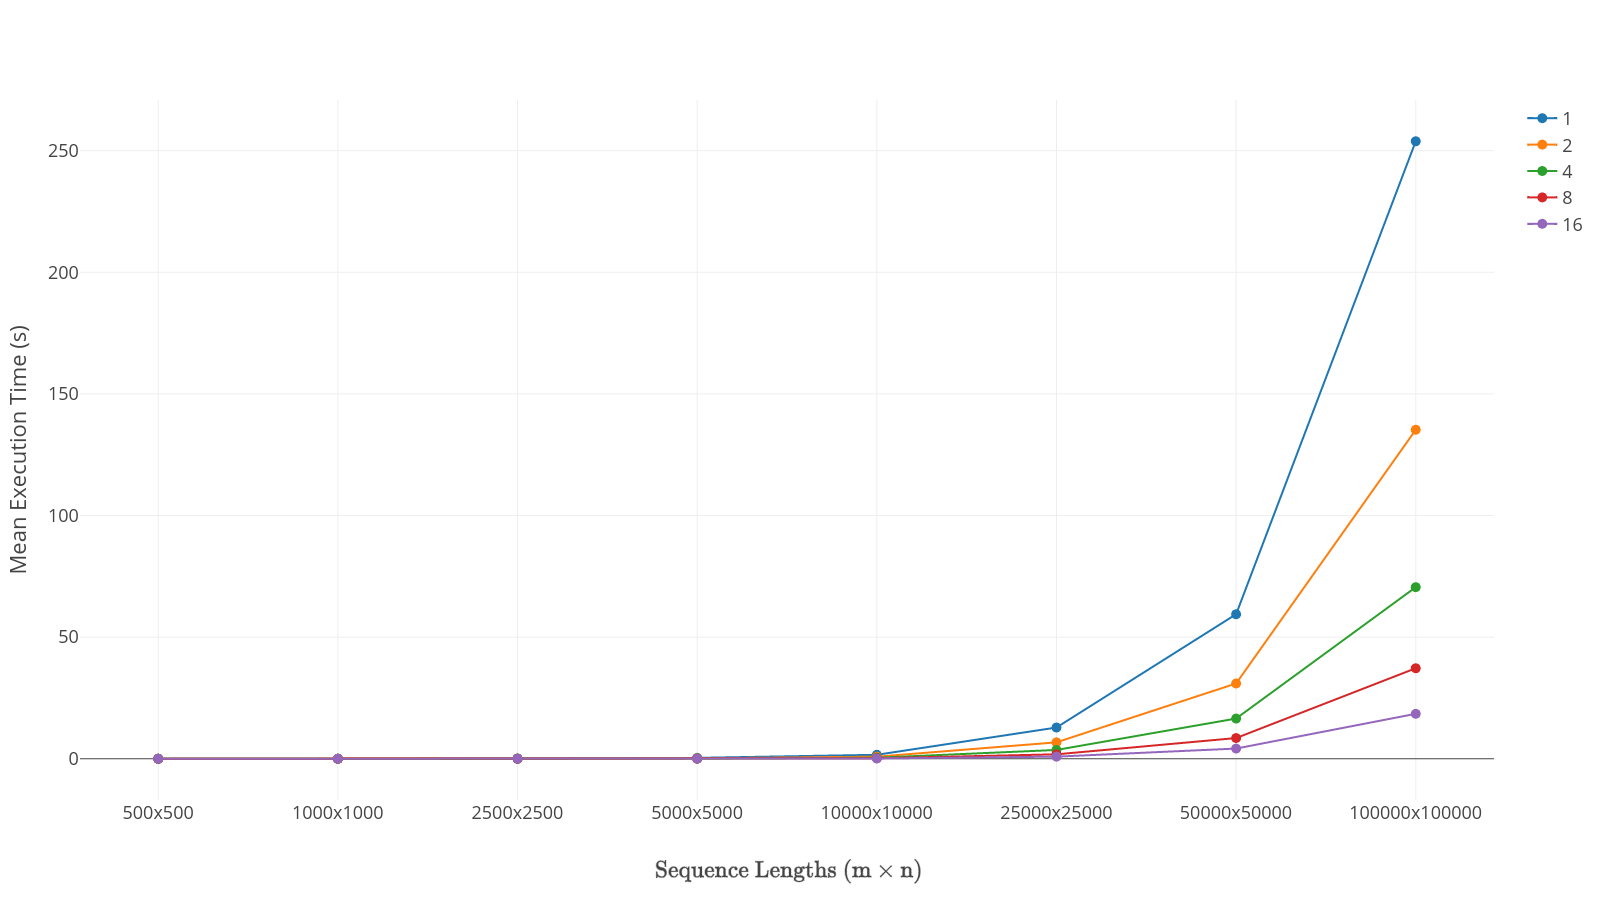
\includegraphics[width=1\textwidth]{equal_txmn.png}
                \caption{Plot of
                $\text{log}_{10}(\text{t}_{\text{exec}})$ against sequence
                lengths, $m,n$, where $m=n$.} \label{equal}
            \end{center}
        \end{figure}

        Note the lengths of the sequences do not necessarily follow a constant
        pattern (they increase in factors of \{2, 2.5, 2, 2, 2.5, 2, 2\}), due
        to timing constraints of the job queue of Slurm. Also note that since
        the execution times increase exponentially, differentiating between the
        functions becomes difficult. Figure \ref{equal_log} provides a semi-
        logarithmic plot of the same data, representing the dependent variable
        in a logarithmic scale.

        \begin{figure}[ht]
            \begin{center}
                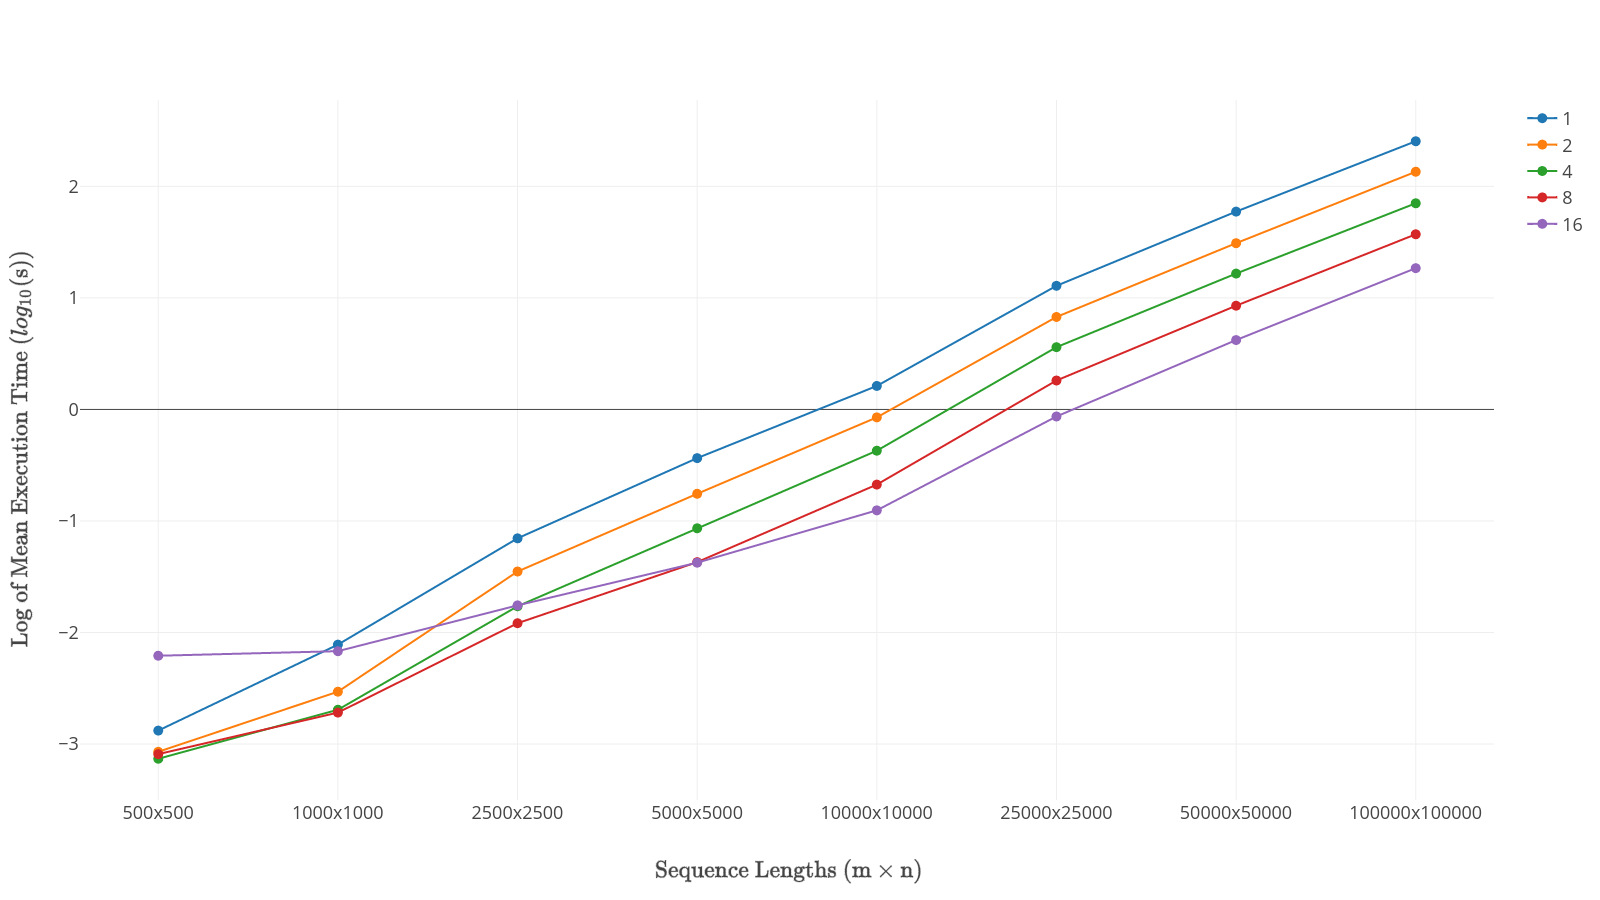
\includegraphics[width=1\textwidth]{equal_log_txmn.png}
                \caption{Semi-logarithm plot of
                $\text{log}_{10}(\text{t}_{\text{exec}})$ against sequence
                lengths, $m,n$, where $m=n$.} \label{equal_log}
            \end{center}
        \end{figure}

        \begin{figure}[ht]
            \begin{center}
                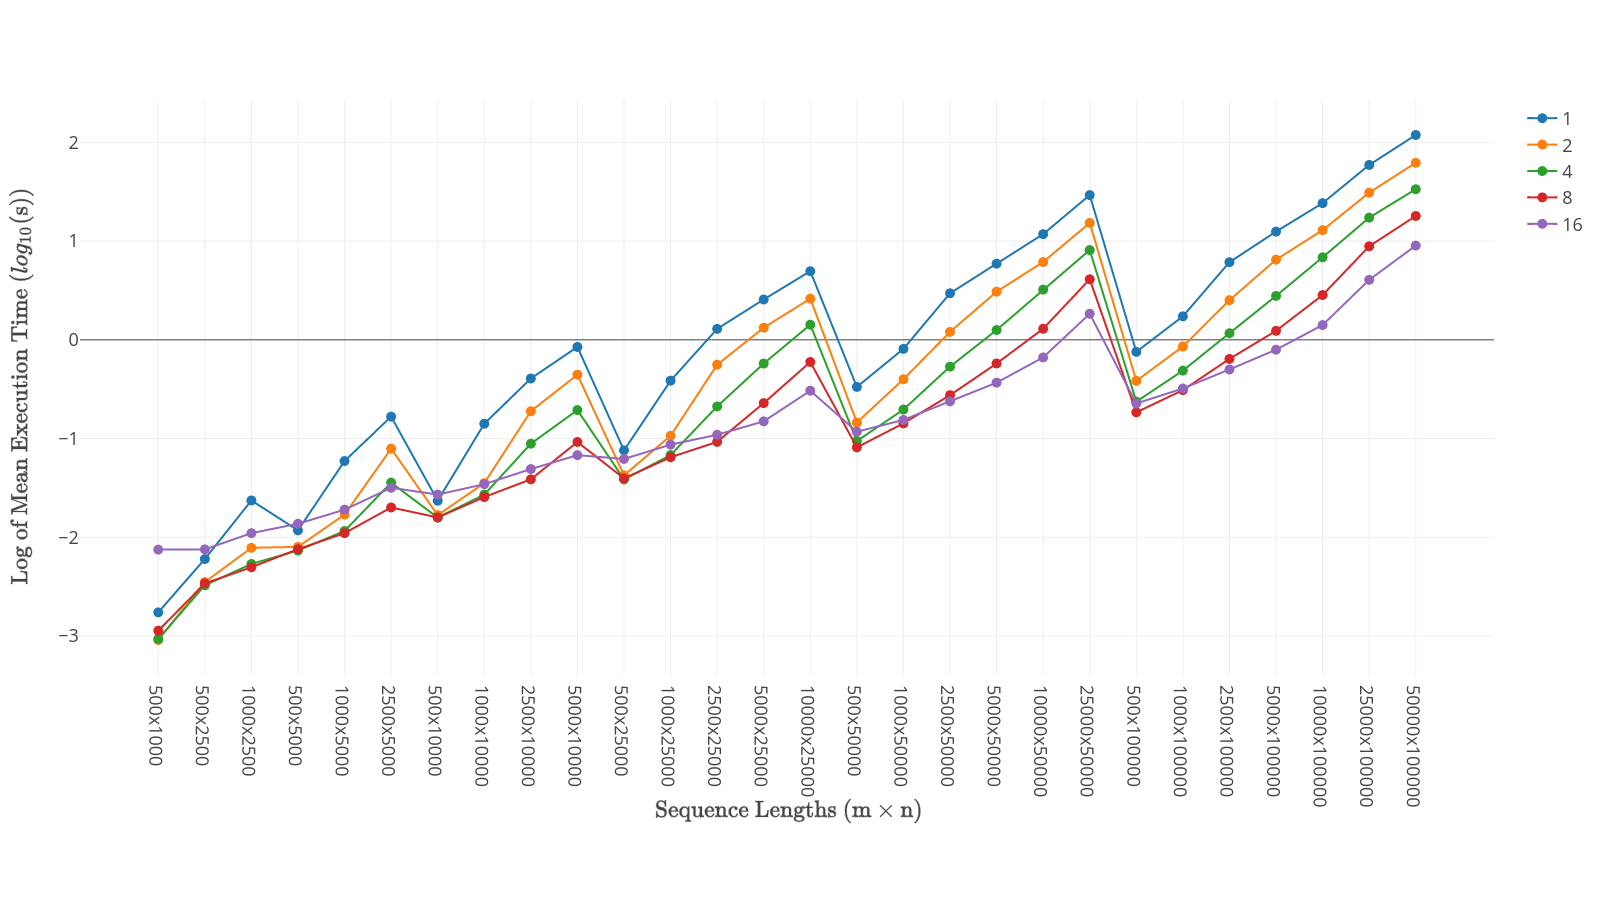
\includegraphics[width=1\textwidth]{unequal_txmn.png}
                \caption{Semi-logarithm plot of
                $\text{log}_{10}(\text{t}_{\text{exec}})$ against sequence
                lengths, $m,n$, where $m\ne n$. } \label{equal}
            \end{center}
        \end{figure}



    \clearpage
    \newpage
    \section{Testing and Debugging} 

        \subsection{Milestone 1} The source code was initially developed in
        C++, but later translated to C. The Intel C++ Compiler, \texttt{icpc},
        did not appear to properly compile the source code. The executable
        built without any warnings or errors, but the algorithm during its
        execution appeared to skip steps. The current implementation in C
        compiles with both \texttt{gcc} and the Intel C Compiler, \texttt{icc}.

        \subsection{Milestone 2} Measurement of the empirical running times
        began using Slurm on the Maya clusters. Initially, the batch submission
        script did not have sufficient memory to compute the LCS of 100,000
        $\times$ 100,000 character length sequences. The memory had to be
        increased by declaring \texttt{\#SBATCH --mem=50000} on the script's
        preprocessor directives. The mean of the execution times for 1, 2, 4, 8
        and 16 cores on the \texttt{hpcf2013} nodes were computed successfully.

    \newpage
    \bibliography{algo,journal_parallel}

\end{document}
